\section{Exact computation, construction, and verification}
\label{sec:computation}

\subsection{Evaluating a likelihood}

The accompanying \texttt{code/compression.py} takes $q,n,H_1,H_0,A$ as JSON data. It validates the two alternating forms, computes the three invariants, and returns the exact rational probability, the joint intersection law, the likelihood relative to independent uniform entries, and the minimum ambient dimension. Field arithmetic is implemented for prime fields and for $\F_4=\F_2[x]/(x^2+x+1)$. The theoretical formulas apply to every prime power; the supplied field implementation does not silently substitute modular arithmetic for other extension fields.

The count of one matrix does not enumerate the group or all possible observations. Gaussian elimination computes the invariants. At most $O((a+b)^2)$ terms of integer arithmetic evaluate the positive sums. This is an arithmetic-operation statement: bit lengths grow with the parameters. Enumerating the \emph{entire} law by listing all matrices still takes $q^{ab}$ observations; we make no polynomial-time claim for that different task.

\subsection{Constructing a smallest realization}

The minimum in Theorem~\ref{thm:minimum-dimension} is attained by an explicit procedure. Write
$R=R_1\oplus R_0\oplus C$, where $R_i=R\cap E_i$, and choose bases $u_i$ of $R_1$ and $v_i$ of $R_0$. Set
\[
 L=\operatorname{span}\{u_i+v_i:1\le i\le\min(t_0,t_1)\}\oplus C.
\]
It has dimension $r-\max(t_0,t_1)$ and meets neither coordinate summand. A symplectic Gram--Schmidt procedure gives hyperbolic pairs for the nondegenerate part of $\Gamma_A$. Complete $L$ to a basis of the radical. Map the hyperbolic pairs to standard symplectic pairs, map $L$ to zero, and map the remaining radical basis vectors to independent isotropic vectors in an additional $2\max(t_0,t_1)$ coordinates. Expressing this map in the original basis produces the two required frames.

The file \texttt{code/minimal\_realization.py} implements this construction and verifies its output by exact field arithmetic. The certificate contains the two frames and the ambient form, so that the identities
\[
 Y^{\mathsf T}JY=H_1,\qquad X^{\mathsf T}JX=H_0,
 \qquad Y^{\mathsf T}JX=A,
\]
and the individual injectivity assertions can be checked directly. Together with the proved lower bound, these identities certify optimality.

\subsection{Independent finite checks}

The main check enumerates prescribed-Gram source frames directly, fixes a target frame, and counts both observed matrices and intersection dimensions. This construction is independent of the transverse-kernel formula. It compares every observation with the exact formula, including those with probability zero.

\begin{center}
\begin{tabular}{@{}lr@{}}
\toprule
Main direct-enumeration verification & Count\\
\midrule
Parameter configurations & 33\\
Matrix values checked & 2,305\\
Joint matrix/intersection cells checked & 4,279\\
Enumerated source-frame instances across configurations & 48,726\\
\bottomrule
\end{tabular}
\end{center}

The suite covers all admissible frame types through dimension three in a four-dimensional binary space, odd-characteristic cases over $\F_3$, and genuine extension-field calculations over $\F_4$. It also includes a full-dimensional target and a larger ambient space. The total counts are recorded in \texttt{results/complete\_law.json}; repeated source frames across configurations are counted as instances, not as distinct objects.

A separately written checker enumerates 3,614 actual subspaces and makes 667 exact parameter comparisons for the radical-transversality formula and its support bound. It covers radical dimensions through six over $\F_2$, four over $\F_3$, and three over $\F_5$. Its output is \texttt{results/radical\_transversality.json}. A second frame implementation checks 1,213 matrix values against 5,574 directly enumerated frames. Exact integer-polynomial arithmetic verifies the asymptotic coefficient and the two-plane rational identities in 388 matrix cases. The minimum-dimension constructor passes 805 exhaustive cross-matrix cases and 12 further edge cases. The programs and their recorded outputs are included.

These checks serve two purposes: they test the normalization and the delicate graph-count factor, and they exercise degenerate forms and characteristic two. The all-parameter mathematical proof is given above. The new theorem has not been formalized or checked in Lean; a dependency-by-dependency formalization blueprint is included separately.

\subsection{An exact numerical example}

Take $q=3$, $n=2$, and two symplectic two-frames, so $H_1=H_0=\left(\begin{smallmatrix}0&1\\-1&0\end{smallmatrix}\right)$. There are 81 possible $2\times2$ observations. The formulas of Section~\ref{sec:asymptotics} give:

\begin{center}
\begin{tabular}{@{}lrrr@{}}
\toprule
Observation class & Matrices & Probability per matrix & Total mass\\
\midrule
$\det A=1$ & 24 & $11/720$ & $11/30$\\
$\det A\ne1$ & 57 & $1/90$ & $19/30$\\
Uniform model, every matrix & 81 & $1/81$ & $1$\\
\bottomrule
\end{tabular}
\end{center}

In particular, $I_2$ and $\operatorname{diag}(1,2)$ have equal rank but different probabilities. Their smallest realization dimensions are respectively two and four. The exact full total variation distance is $19/270$. Thus both probability and realizability see structure that ordinary matrix rank misses.

\begin{figure}[htbp]
\centering
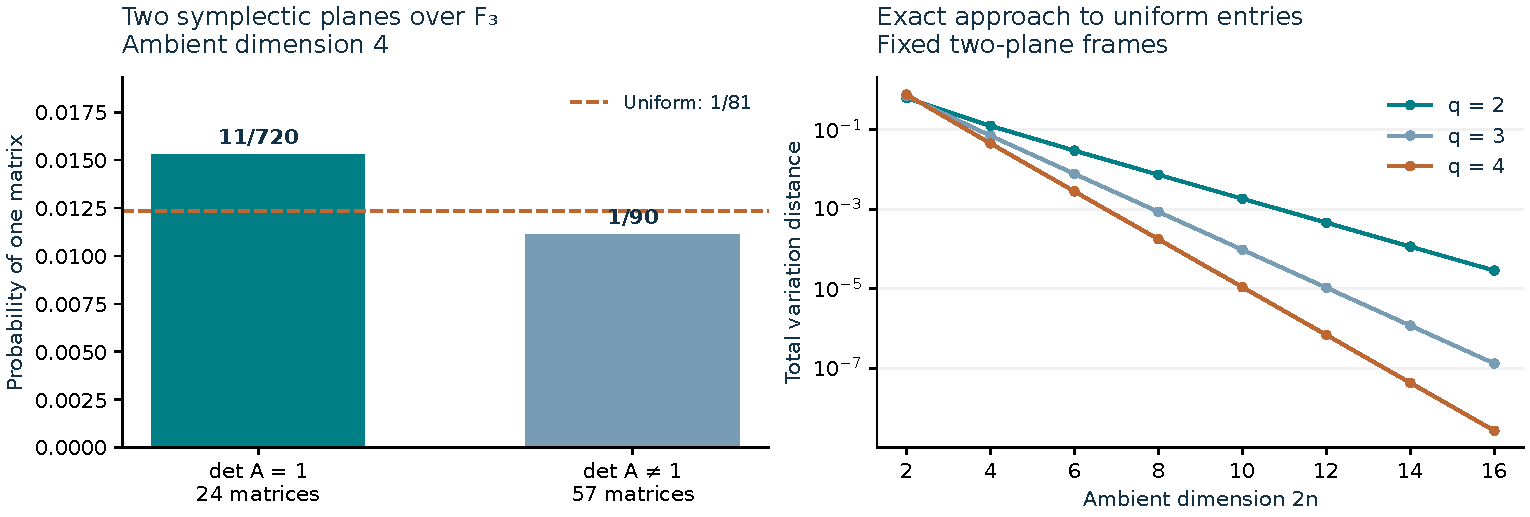
\includegraphics[width=\linewidth]{figures/two_plane_law.pdf}
\caption{Exact two-plane laws. Left: per-matrix probabilities for the example over $\F_3$ in ambient dimension four. Right: the exact total variation distance as the ambient dimension increases; the sharp rate is $q^{-2n}$. Lines connect exact finite formulas and are not Monte Carlo estimates.}
\label{fig:two-plane}
\end{figure}
